{
{\sffamily I det følgende vil vi samle op på resultaterne fra det kørte
eksperiment med den naive vurdering af regioner. Vores metode til
udtrækning af regioner, har dog indeholdt en fejl, som vi først vil
beskrive.
}

\subsection{Systematisk fejl\label{program_bug}}
I den naive løsning findes en fejl i udtrækningen af regioner, som gør
at vi finder nogle af
regionerne flere gange. Denne fejl nævnt i afsnit
\ref{section_impBilledbehandling} og gennemgået i bilag
\ref{appendix_bug}. Det betyder, at de resultater vi fremviser for kørslen
af den naive løsning, ikke helt passer. For at give en indblik i, hvor
mange regioner der bliver fundet flere gange, har vi afprøvet programmet med
fejlen på 11 malerier, og sammenlignet dem med en kørsel, hvor fejlen er
rettet.

De 11 malerier er opstillet i tabel \ref{bug_tabel}, hvor de to første
kolonner er antal regioner fundet i billedet, uden og med fejl.  Tredje
kolonne er en procentsats for, hvor mange flere regioner der bliver
fundet, når den fejlende kode køres. Den procentvise spredning er $[60
\%,~377 \%]$, så de resultater vi får, kan være op til $377\%$ for høje.
Gennemsnitligt er der $172 \%$ flere regioner. Vi kan godt antage, at
antallet af regioner opgivet i resultaterne for den naive løsning, er
halv så store.

\begin{table}[!h]
    \centering
    \begin{tabular}{|l|c|c|c|}
        \hline
  Maleri  & Bug løst 		& Bug ikke løst		& Procentvis forskel\\\hline
        1   & 70 			& 112 				& 60 \% \\
        2   & 27 			& 45 				& 67 \% \\
        3	& 52 			& 98 				& 72 \% \\
        4   & 84 			& 145 				& 73 \% \\
        5	& 32 			& 57 				& 78 \% \\
        6   & 88 			& 170 				& 93 \% \\
        7   & 85 			& 201 				& 136 \% \\
        8   & 78 			& 197 				& 153 \% \\
        9   & 164 			& 554 				& 238 \% \\
        10	& 16 			& 75 				& 368 \% \\
        11	& 115 			& 548 				& 377 \% \\\hline
	Total	& 881			& 2202				& 172 \% \\\hline
	  \end{tabular}
    \caption[]{Tabel for antal fundne regioner i versionen med og uden
    fejlen som duplikerer regioner. Den sidste kolonne er hvor mange
    procent flere regioner der bliver fundet.}
    \label{bug_tabel}
\end{table}

\clearpage

\subsection{Resultater}
Vi har kørt analyse med naiv vurdering på $17,364$ malerier, men i vores
resultater sorterer vi $2,989$ af disse fra, da de kun er udsnit af et
større maleri.  Som vist i tabel \ref{tabel_fjern_detaljer} herunder, er
dette en nedgang på $17.21$ procent og vi har $14,375$ brugbare
resultater tilbage.

\begin{table}[H]
    \centering
    \begin{tabular}{r@{\ \ }p{12em}r|r@{.}l}
            & Analyserede malerier & $17,364$ & $100$ & $00\%$   \\
        $-$ & Udsnit af malerier   &  $2,989$ &  $17$ & $21\%$   \\\hline
            & Resultater           & $14,375$ &  $82$ & $79\%$
    \end{tabular}
    \caption[]{Udregning af brugbare resultater.}
    \label{tabel_fjern_detaljer}
\end{table}

Af de brugbare resultater, ser vi i tabel \ref{tabel_fordeling}, at der
i $91.43$ procent af malerierne er fundet mindst én region som ligger i
det gyldne snit. Vi kan derfor ikke afvise hypotese \ref{hypo_binaer}.

\begin{table}[H]
    \centering
    \begin{tabular}{r@{\ \ }p{12em}r|r@{.}l}
            & Positive resultater   & $13,143$ &  $91$ & $43\%$ \\
        $+$ & Negative resultater   &  $1,232$ &   $8$ & $57\%$ \\\hline
            & Resultater i alt      & $14,375$ & $100$ & $00\%$
    \end{tabular}
    \caption[]{Et positivt resultat beskriver et maleri, hvori der er
    fundet mindst én region, som ligger i det gyldne snit. Et negativt
    resultat er et maleri, hvori der ikke findes nogen regioner, som
    ligger i det gyldne snit.}
    \label{tabel_fordeling}
\end{table}

Vi vil gerne se på, hvordan fordelingen af fundne interessante regioner i
de fire gyldne snit ser ud. Fordelingen er vist i tabel
\ref{tabel_fire_snit}. Vi ser, at ingen af snittene afviger med mere end
$\pm10\%$ fra et andet og vi kan derfor ikke afvise hypotese
\ref{hypo_fire_g_snit}.

\begin{table}[H]
    \centering
    \begin{tabular}{r@{\ \ }p{12em}r|r@{.}l}
            & Regioner i snit 0   &  $42,884$ &  $24$ & $51\%$ \\
        $+$ & Regioner i snit 1   &  $44,042$ &  $25$ & $18\%$ \\
        $+$ & Regioner i snit 2   &  $46,432$ &  $26$ & $54\%$ \\
        $+$ & Regioner i snit 3   &  $41,547$ &  $23$ & $75\%$ \\\hline
            & Regioner i alt      & $168,650$ & $100$ & $00\%$
    \end{tabular}
    \caption[]{Forholdet mellem de interessante regioner fundet i de
    fire gyldne snit. Intet snit afviger med mere end $10\%$ fundne
    regioner, end et andet snit.}
    \label{tabel_fire_snit}
\end{table}

Vi undersøger nu, hvor mange af de brugbare resultater, som er forsynet
med dimensioner i databasen, således at vi kan undersøge, hvorvidt
lærredet er konstrueret som et gyldent rektangel. Udregningen i tabel
\ref{tabel_med_dimensioner} viser at ud af de brugbare resultater,
mangler $2,410$ malerier dimensionerne, og vi har da $11,965$ malerier
tilbage at undersøge, for den gyldne ratio i lærredets dimensioner.

\begin{table}[H]
    \centering
    \begin{tabular}{r@{\ \ }p{14em}r|r@{.}l}
            & Resultater                     & $14,375$ & $100$ & $00\%$ \\
        $-$ & Resultater uden dimensioner    &  $2,410$ &  $16$ & $77\%$ \\\hline
            & Resultater med dimensioner     & $11,965$ &  $83$ & $23\%$
    \end{tabular}
    \caption[]{Brugbare resultater med dimensioner i databasen.}
    \label{tabel_med_dimensioner}
\end{table}

Vi ser nu, hvor mange af de $11,965$ malerier, der har, at dets lange
side, $L$, divideret med dets korte side, $K$, ligger i intervallet $G =
[1.57920117302, 1.65686680448] = \varphi \pm 2.4\%$. Tabel
\ref{tabel_real_dimensions} viser, at kun $3.99\%$ falder inden for
dette interval. Vi kan således afvise hypotese
\ref{hypo_golden_ractangle}.

\begin{table}[H]
    \centering
    \begin{tabular}{r@{\ \ }p{14em}r|r@{.}l}
            & $L/K \in G$                  &    $478$ &   $3$ & $99\%$ \\
        $+$ & $L/K \notin G$               & $11,487$ &  $96$ & $01\%$ \\\hline
            & Resultater med dimensioner   & $11,965$ & $100$ & $00\%$
    \end{tabular}
    \caption[]{Resultater med dimensioner, hvor disse er et gyldent
    rektangel med en afvigelse på $2.4\%$. Under en tredjedel af
    malerierne har et lærred med gyldne dimensioner.}
    \label{tabel_real_dimensions}
\end{table}

\begin{table}[H]
    \centering
    \begin{tabular}{|c|l|c|c|}
        \textbf{Hypotese nr.} & \textbf{Beskrivelse} & \textbf{Afvist} &
        \textbf{Ikke afvist}  \\\hline\hline
        1 & Mindst én region i $GS$                     &            & \checkmark   \\\hline
        2 & Alle fire $GS$ lige meget brugt             &            & \checkmark   \\\hline
        3 & $1/3$ har lærred med forholdet $1:\varphi $ & \checkmark &              \\\hline
        4 & Flest regioner i $GS$                       & \checkmark &              \\\hline
        5 & Flere regioner i $GS$ end $\frac{2}{3}$     &            & \checkmark   \\\hline
        6 & Flere regioner i $GS$ end i midten          & \checkmark &              \\\hline
        7 & $GS$ brugt lige meget, uanset tidsperiode   &            &              \\\hline
        8 & $GS$ brugt lige meget, uanset nationalitet  &            &              \\\hline
        9 & $\frac{2}{3}$ brugt som approksimation til $GS$   &            & \checkmark	\\\hline
    \end{tabular}
    \caption[]{Hypoteser i forhold til den naive kørsel. $GS$ bruges som
    forkortelse for det gyldne snit.}
    \label{hypoteser_naiv}
\end{table}

\subsubsection{Antallet af fundne regioner over alle snit}
I alle $14,375$ malerier er der i alt fundet $1,650,082$ interessante
regioner. Vi har en middelværdi på $114.79$ med standardafvigelse på
$86.91$. I figur \ref{total_regions_plots} er vist grafer over hvordan
antallet af fundne regioner fordeler sig i malerierne. I figur
\ref{graf_total_regions_zoom}, hvor der ses bort fra $298$ malerier,
hvori der ikke er fundet nogen regioner. Regionerne i malerierne har en
fordeling, der kunne ligne en eksponentialfordeling, som vist i
histogrammet i figur \ref{hist_total_regions}. De observerede værdier
fraviger dog noget fra de teoretiske værdier.

\begin{figure}[!h]
    \centering
    \subfloat[]{
        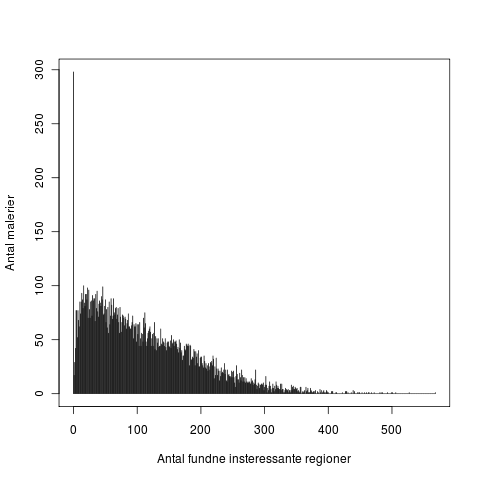
\includegraphics[width=0.49\textwidth]{afsnit/resultater/billeder/totalregions_var}
        \label{graf_total_regions_var}
    }
    \subfloat[]{
        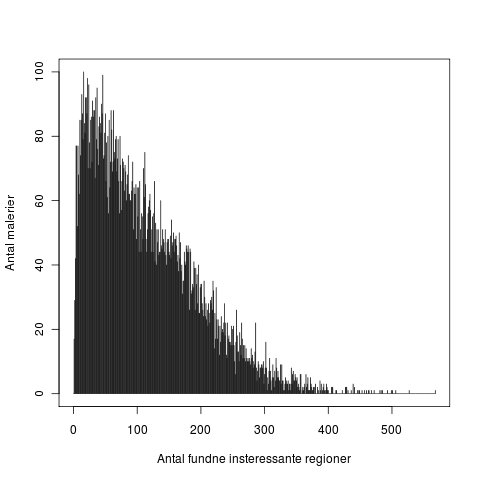
\includegraphics[width=0.49\textwidth]{afsnit/resultater/billeder/totalregions}
        \label{graf_total_regions_zoom}
    }\\
    \subfloat[]{
        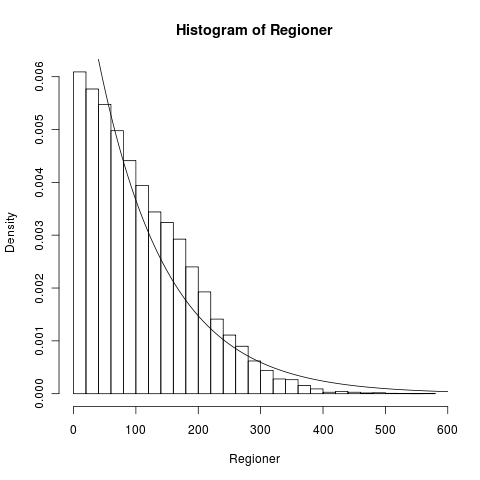
\includegraphics[width=0.62\textwidth]{afsnit/resultater/billeder/hist_totalregions}
        \label{hist_total_regions}
    }
    \caption[]{Fordelingen af fundne regioner på malerier.
    \textbf{\ref{graf_total_regions_var}:} Plot som viser hvor mange
    malerier, hvori der er fundet et vist antal interessante regioner
    over alle snit i maleriet.  \textbf{\ref{graf_total_regions_zoom}:}
    Samme plot som i figur \ref{graf_total_regions_var}, men hvor antal
    malerier uden regioner ikke er vist.
    \textbf{\ref{hist_total_regions}:} Histogram over antal fundne
    regioner, hvor en eksponentialfordeling med $\lambda = 1/109.82$ er
    indtegnet.}
    \label{total_regions_plots}
\end{figure}

Vi ser, at et maleri typisk har omkring $110$ interessante regioner i
alle snit. Her skal man være opmærksom på, at hver region meget vel
indgår fire gange. Vi ser, at der er et lille antal malerier, hvori der
bliver fundet rigtig mange regioner. Det tynder dog ud omkring
$380$ regioner, hvor antallet af malerier, med flere regioner,
forekommer mindre hyppigt.

Vi skal være opmærksomme på, at der kan være duplikater af regionerne.

}

% vim: set tw=72 spell spelllang=da:
